\documentclass[]{article}
\usepackage{xcolor}
\usepackage{listings}
\usepackage{graphicx}
% \lstset{language=C++,
% 	% numbers=left,
% 	%	stepnumber=1,
% 	numberstyle=\ttfamily,
% 	basicstyle=\ttfamily,
% 	keywordstyle=\color{blue}\ttfamily,
% 	stringstyle=\color{red}\ttfamily,
% 	commentstyle=\color{gray}\ttfamily,
% 	morecomment=[l][\color{magenta}]{\#}
% }

%opening
\title{Tugas 3: Stack}
\author{Azzam Wildan Maulana NRP 5024201010}

\begin{document}{}
\maketitle

\section{Source Code}
Berikut adalah source code dasar yang saya buat
\lstinputlisting{stack.c}
Disana saya membuat stack dengan C serta fungsi-fungsi untuk push dan pop.
\\
%No 1
% \subsection{Desain Struktur Data}
% Struktur data saya simpan pada Class DBKota
% \lstinputlisting{1.cpp}
% Dia memiliki method method dasar seperti tambah, hapus, tampilkan, dan cari.
% \\

%No 2
% \subsection{Fungsi untuk menambahkan data kota ke dalam suatu array}
% \lstinputlisting{2a.cpp}
% Saya membuat fungsi bernama append, Dia menerima variabel yang digunakan untuk mengisi struct kota_t.
% \\
% \subsection{Fungsi untuk menyisipkan dan menghapus kota tersebut kedalam array}
% \lstinputlisting{2b.cpp}
% Untuk menyisipkan data, saya pakai fungsi insert sedangkan untuk menghapus data saya pakai remove
% \\
% \subsection{Fungsi untuk mencari nama kota, output dari fungsi tersebut adalah index array kota tersebut}
% \lstinputlisting{2c.cpp}
% Untuk mencari nama kota, saya pakai fungsi searchByName. Dia akan mencari dengan metode linear search dan jika ketemu langsung di-return kan posisinya. 
% \\
% \subsection{Output Program}
% 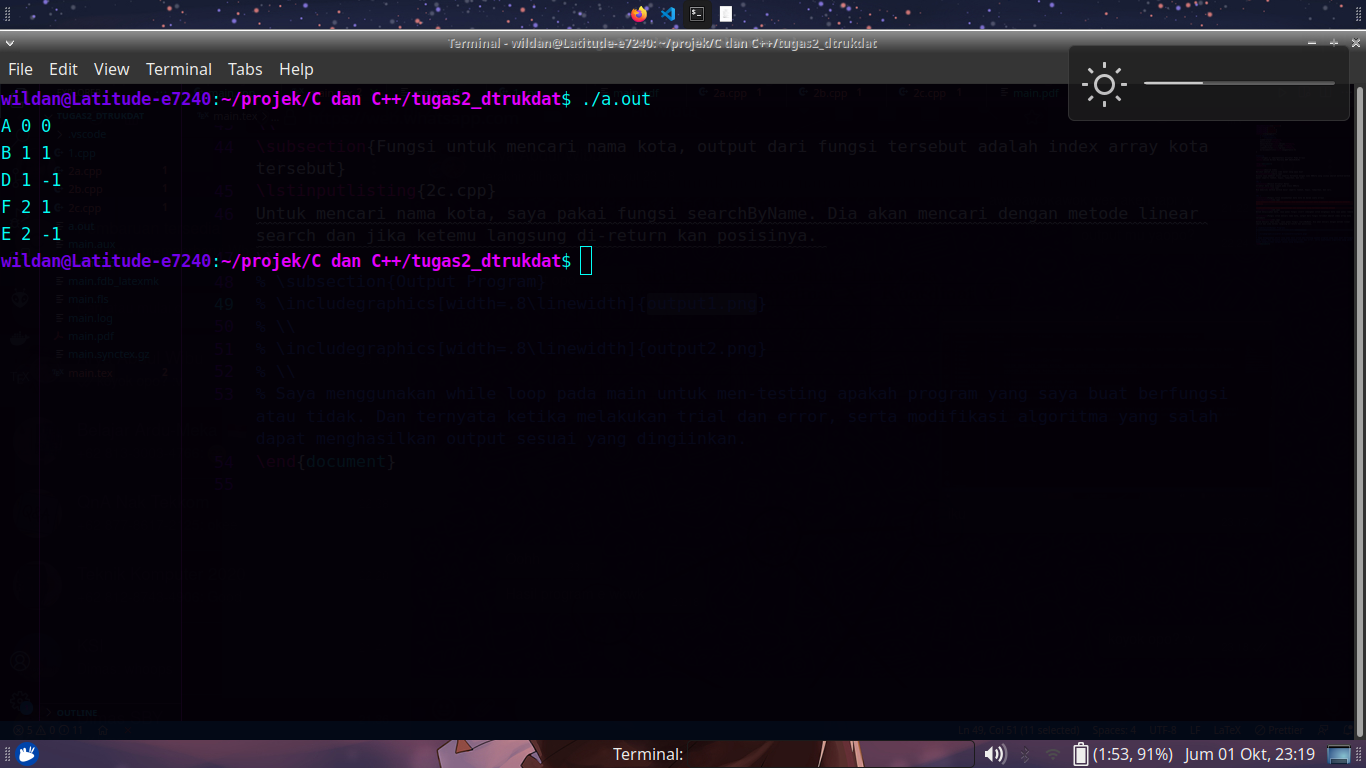
\includegraphics[width=.8\linewidth]{output.png}
% \\
% \includegraphics[width=.8\linewidth]{output2.png}
% \\
% Saya menggunakan while loop pada main untuk men-testing apakah program yang saya buat berfungsi atau tidak. Dan ternyata ketika melakukan trial dan error, serta modifikasi algoritma yang salah dapat menghasilkan output sesuai yang dingiinkan.
\end{document}
